\documentclass[11pt]{beamer}
\usepackage{bm,booktabs,mmacells,minted,tabularx}
% \usepackage{auto-pst-pdf,float,pstricks}
\usetheme{AnnArbor}
\setbeamercolor{normal text}{bg=black!10}
\definecolor{bg}{rgb}{0.95,0.95,0.95}
\usemintedstyle{emacs}
\newcommand{\executeiffilenewer}[3]{%
    \ifnum\pdfstrcmp{\pdffilemoddate{#1}}%
    {\pdffilemoddate{#2}}>0%
    {\immediate\write18{#3}}\fi%
}
\newcommand{\includesvg}[2]{%
    \executeiffilenewer{#2.svg}{#2.pdf}%
    {inkscape -D --export-filename=#2.pdf #2.svg}%
    \includegraphics[width=#1]{#2.pdf}%
}
\begin{document}
\title{Design of Integrated Microrobotic Fish}
\subtitle{Presentation 3 - Physical Model (Improving) \& COMSOL Simulation (Debugging)}
\author{Yihua Liu}
\institute{UM-SJTU Joint Institute}
\date{March 9, 2021}
\maketitle
\begin{frame}{Contents}
    \tableofcontents
\end{frame}
\section{Antecedent}
\begin{frame}[fragile]{Antecedent}{Total Impedance $Z$}
    \begin{mmaCell}{Input}
        R=\mmaFrac{Pi*x*(\mmaSqrt{k}+\mmaFrac{1}{\mmaSqrt{k}})}{2\mmaUnd{\(\pmb{\sigma}\)}*\mmaUnd{\(\pmb{\delta}\)x}};
        \mmaSub{C}{DL}=\mmaFrac{\mmaUnd{\(\pmb{\epsilon}\)}*\mmaUnd{\(\pmb{\delta}\)x}*\mmaSqrt{k}}{\mmaSub{\mmaUnd{\(\pmb{\lambda}\)}}{D}};
        \mmaSub{C}{DS}=\mmaFrac{\mmaUnd{\(\pmb{\epsilon}\)}*\mmaUnd{\(\pmb{\delta}\)x}}{\mmaSqrt{k}*\mmaSub{\mmaUnd{\(\pmb{\lambda}\)}}{D}};
        Zx=R+\mmaFrac{1}{I*\mmaUnd{\(\pmb{\omega}\)}*\mmaSub{C}{DL}}+\mmaFrac{1}{I*\mmaUnd{\(\pmb{\omega}\)}*\mmaSub{C}{DS}}
    \end{mmaCell}
    \begin{mmaCell}[addtoindex=3]{Output}
        \mmaFrac{(\mmaFrac{1}{\mmaSqrt{k}}+\mmaSqrt{k}) \(\pi\) x}{2\(\delta\)x \(\sigma\)}-\mmaFrac{i\mmaSub{\(\lambda\)}{D}}{\mmaSqrt{k} \(\delta\)x\(\epsilon \omega\)}-\mmaFrac{i \mmaSqrt{k} \mmaSub{\(\lambda\)}{D}}{\(\delta\)x \(\epsilon \omega\)}
    \end{mmaCell}
    \begin{mmaCell}[addtoindex=5]{Input}
        Simplify[Zx]
    \end{mmaCell}
    \begin{mmaCell}{Output}
        \mmaFrac{(1+k) (\(\pi\) x \(\epsilon \omega\)-2 i \(\sigma\)\mmaSub{\(\lambda\)}{D})}{2 \mmaSqrt{k} \(\delta\)x \(\epsilon \sigma\omega\)}
    \end{mmaCell}
\end{frame}
\begin{frame}[fragile]{Total Impedance $Z$}
    Remind the formula given in the article
    \[Z=\frac{\pi\left(\sqrt{k}+\frac{1}{\sqrt{k}}\right)}{2l\sigma}\frac{\ln{A}-i\theta}{(\ln{A})^2+\theta^2}\]
    where
    \[A=\frac{\sqrt{\left[\left(2\lambda_D\sigma\right)^2+(\omega\varepsilon\pi)^2+x_{min}x_{max}\right]^2+\left[2\lambda_D\sigma\omega\varepsilon\pi\left(x_{max}-x_{min}\right)\right]^2}}{\left(2\lambda_D\sigma\right)^2+(\omega\varepsilon\pi x_{min})^2}\]
    and\\
    \[\theta=\arctan{\frac{2\lambda_D\sigma\omega\varepsilon\pi\left(x_{max}-x_{min}\right)}{\left(2\lambda_D\sigma\right)^2+(\omega\varepsilon\pi)^2x_{min}x_{max}}}\]
    The author probably made a mistake of $A$. The correct formula is
\end{frame}
\begin{frame}{Total Impedance $Z$}
    \includegraphics[width=0.9\textwidth]{1.eps}
\end{frame}
\begin{frame}{Total Impedance $Z$}
    \includegraphics[width=1\textwidth]{2.eps}
\end{frame}
\begin{frame}{Total Impedance $Z$}
    \begin{columns}[onlytextwidth]
        \begin{column}{0.35\textwidth}
            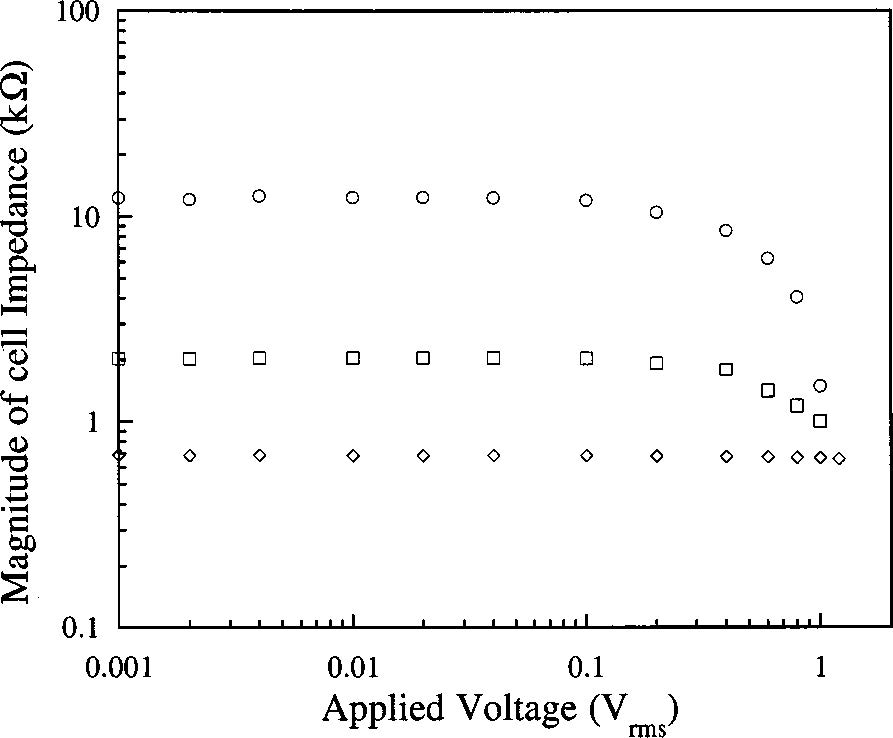
\includegraphics[width=\columnwidth]{6.jpg}
        \end{column}
        \begin{column}{0.6\textwidth}
            Here we restore the resistance to three-dimensional by dividing by the total length of the electrodes in the cell $l=23.5$ cm.\\
            % From the results above, we found that the corrected value of $\mathrm{Re}\{Z\}$ is in the range of 0.1 k$\Omega$ - 1 k$\Omega$ but differs from the value in FIG. 7. of the article.\\
            We again made a mistake here last time. What the paper gives in its FIG. 7. is the magnitude of cell impedance, i.e.,
            \[\mathrm{Abs}[Z]=1430.58\,\Omega\]
            which is closed to the corresponding value in FIG. 7.
            We can directly found that the frequency is not correlated with the applied voltage.\\
            Next, the left side is FIG. 8. in the paper and the right side is our result.
        \end{column}
    \end{columns}
\end{frame}
\begin{frame}{Total Impedance $Z$}
    \begin{columns}[onlytextwidth]
        \begin{column}{0.35\textwidth}
            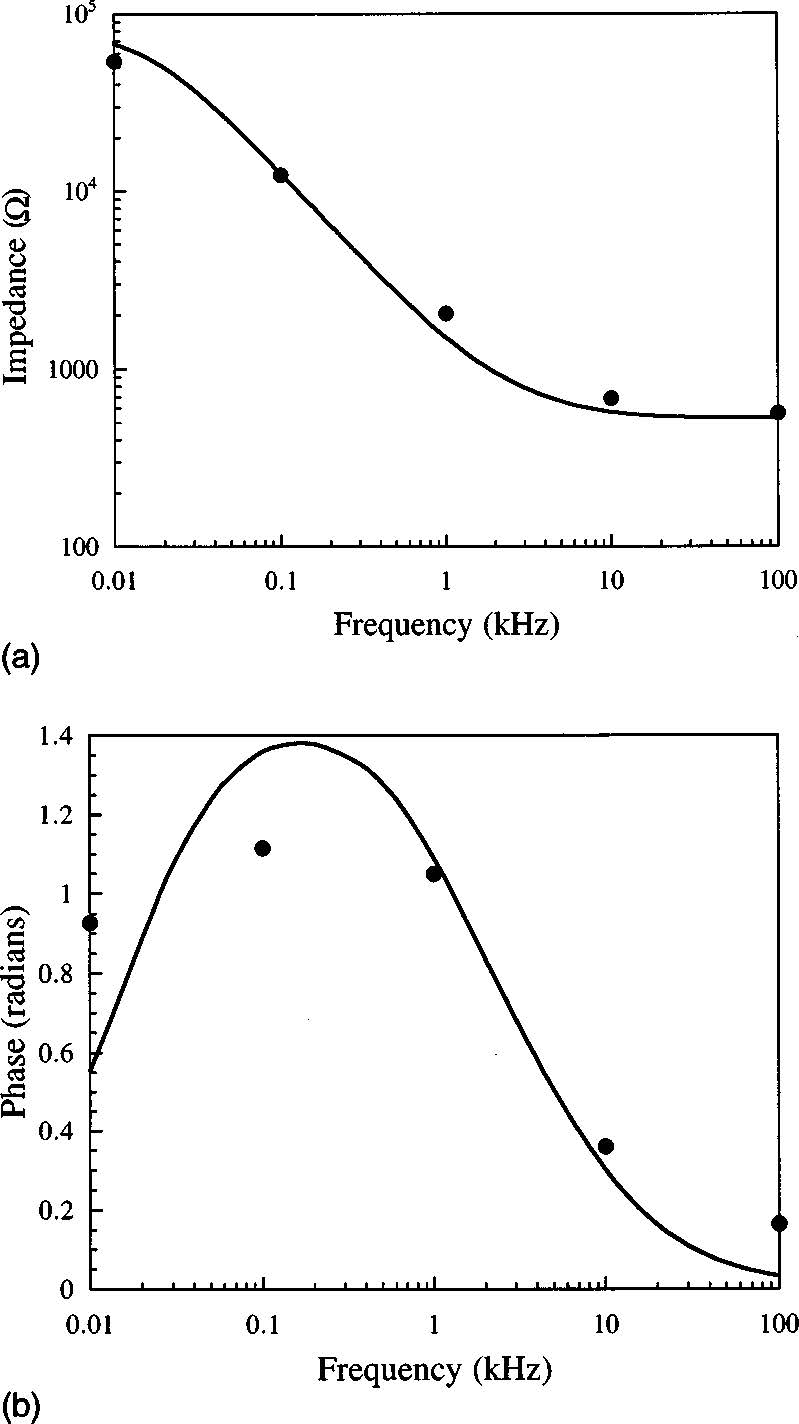
\includegraphics[width=\columnwidth]{5.jpg}
        \end{column}
        \begin{column}{0.6\textwidth}
            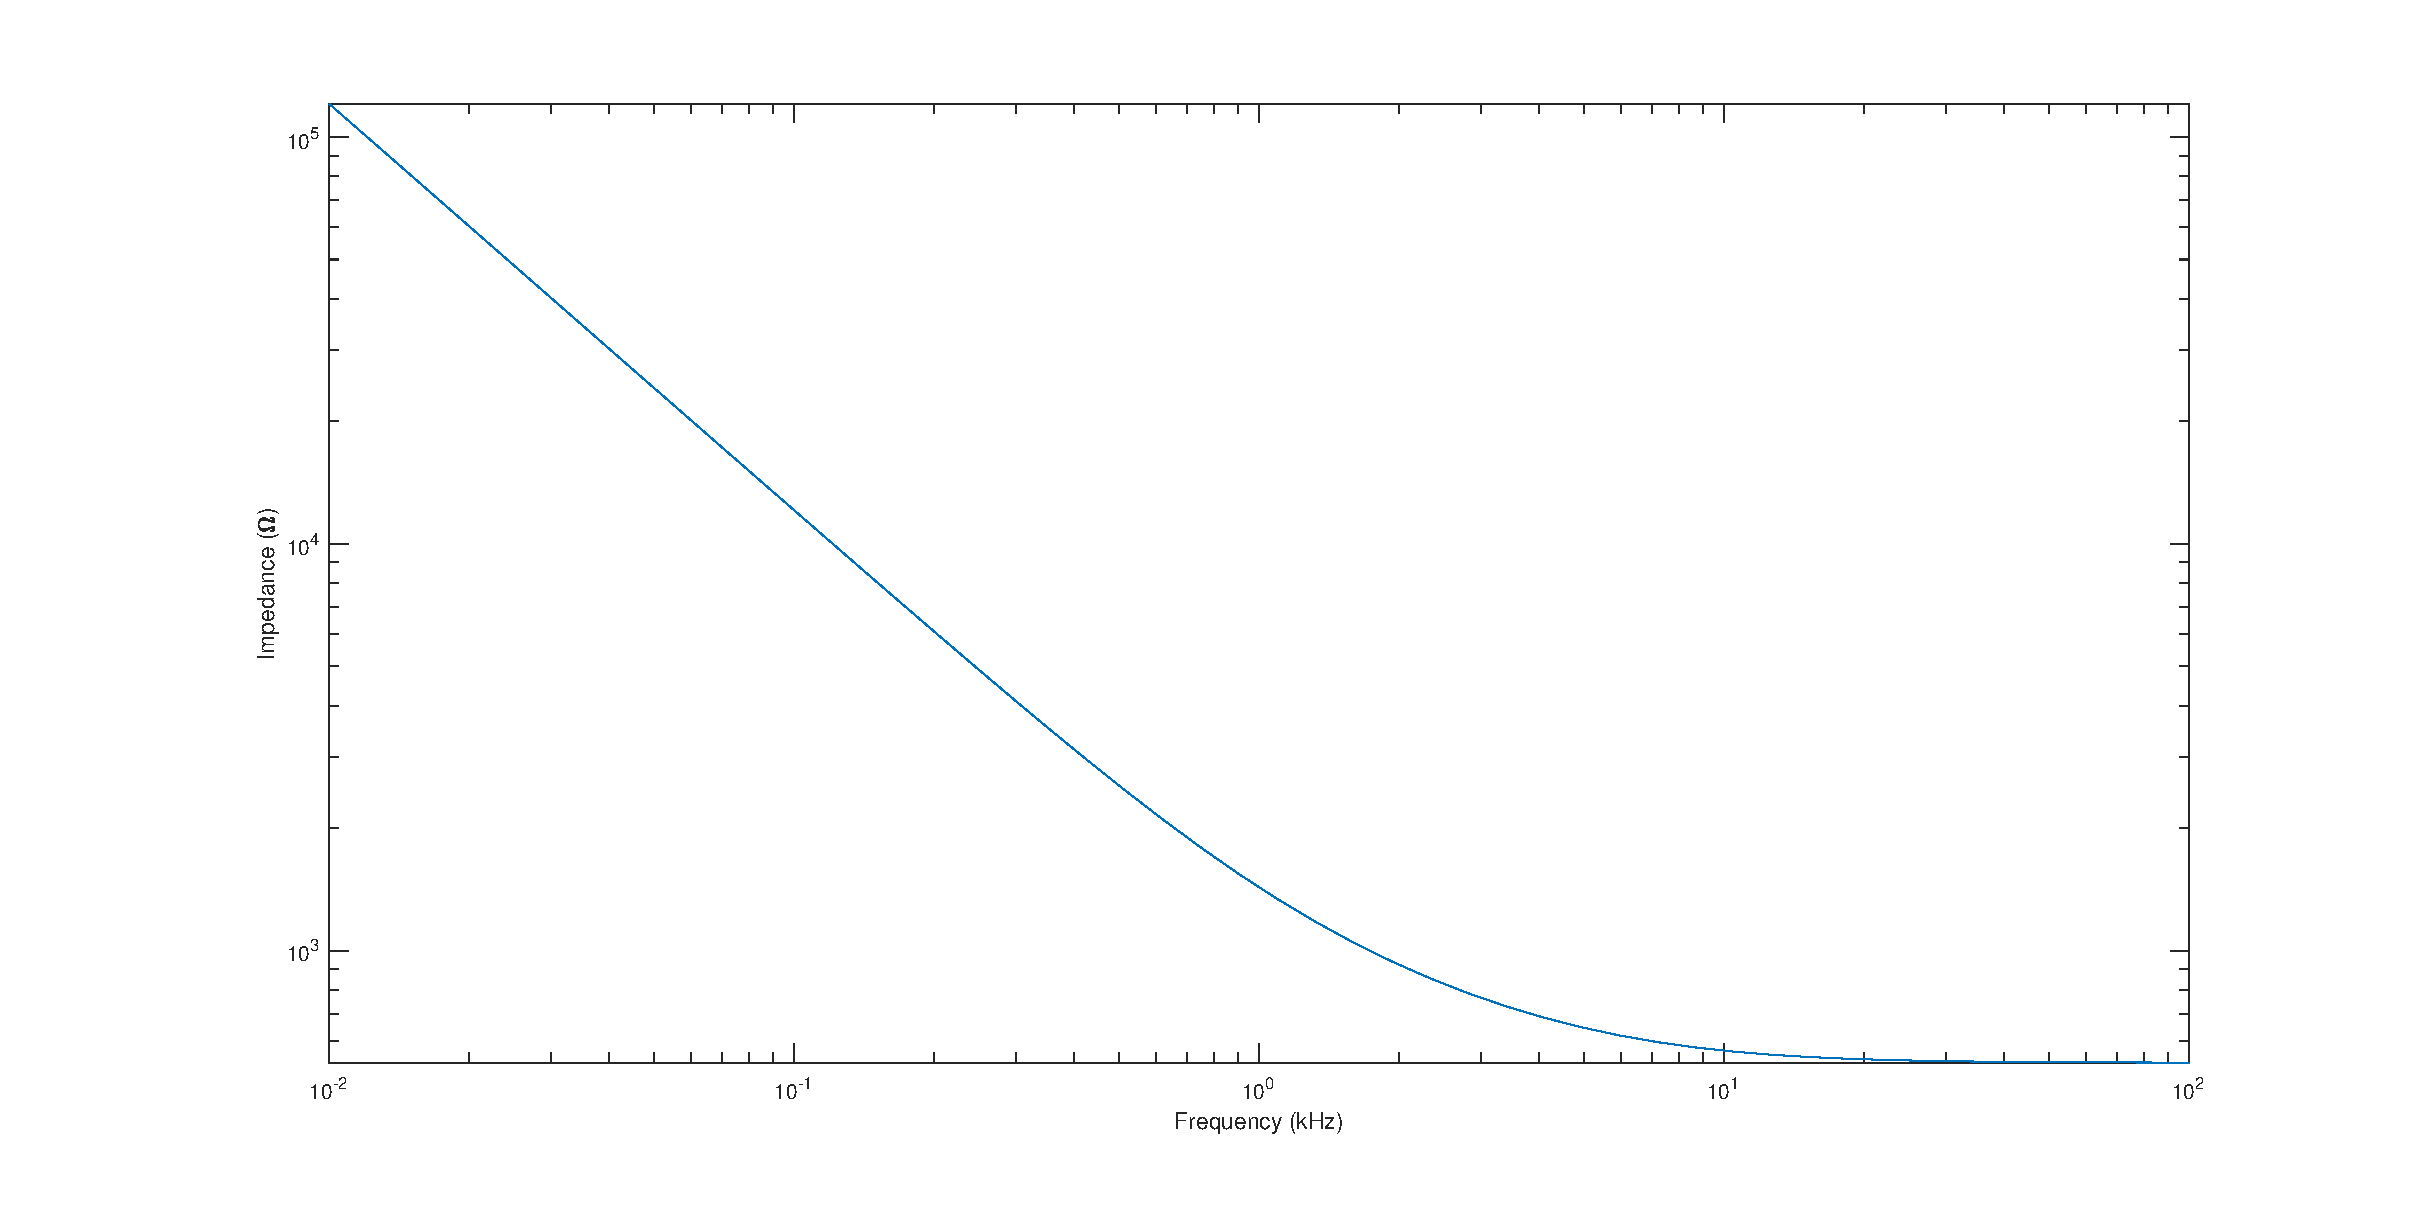
\includegraphics[width=\columnwidth]{3.eps}
            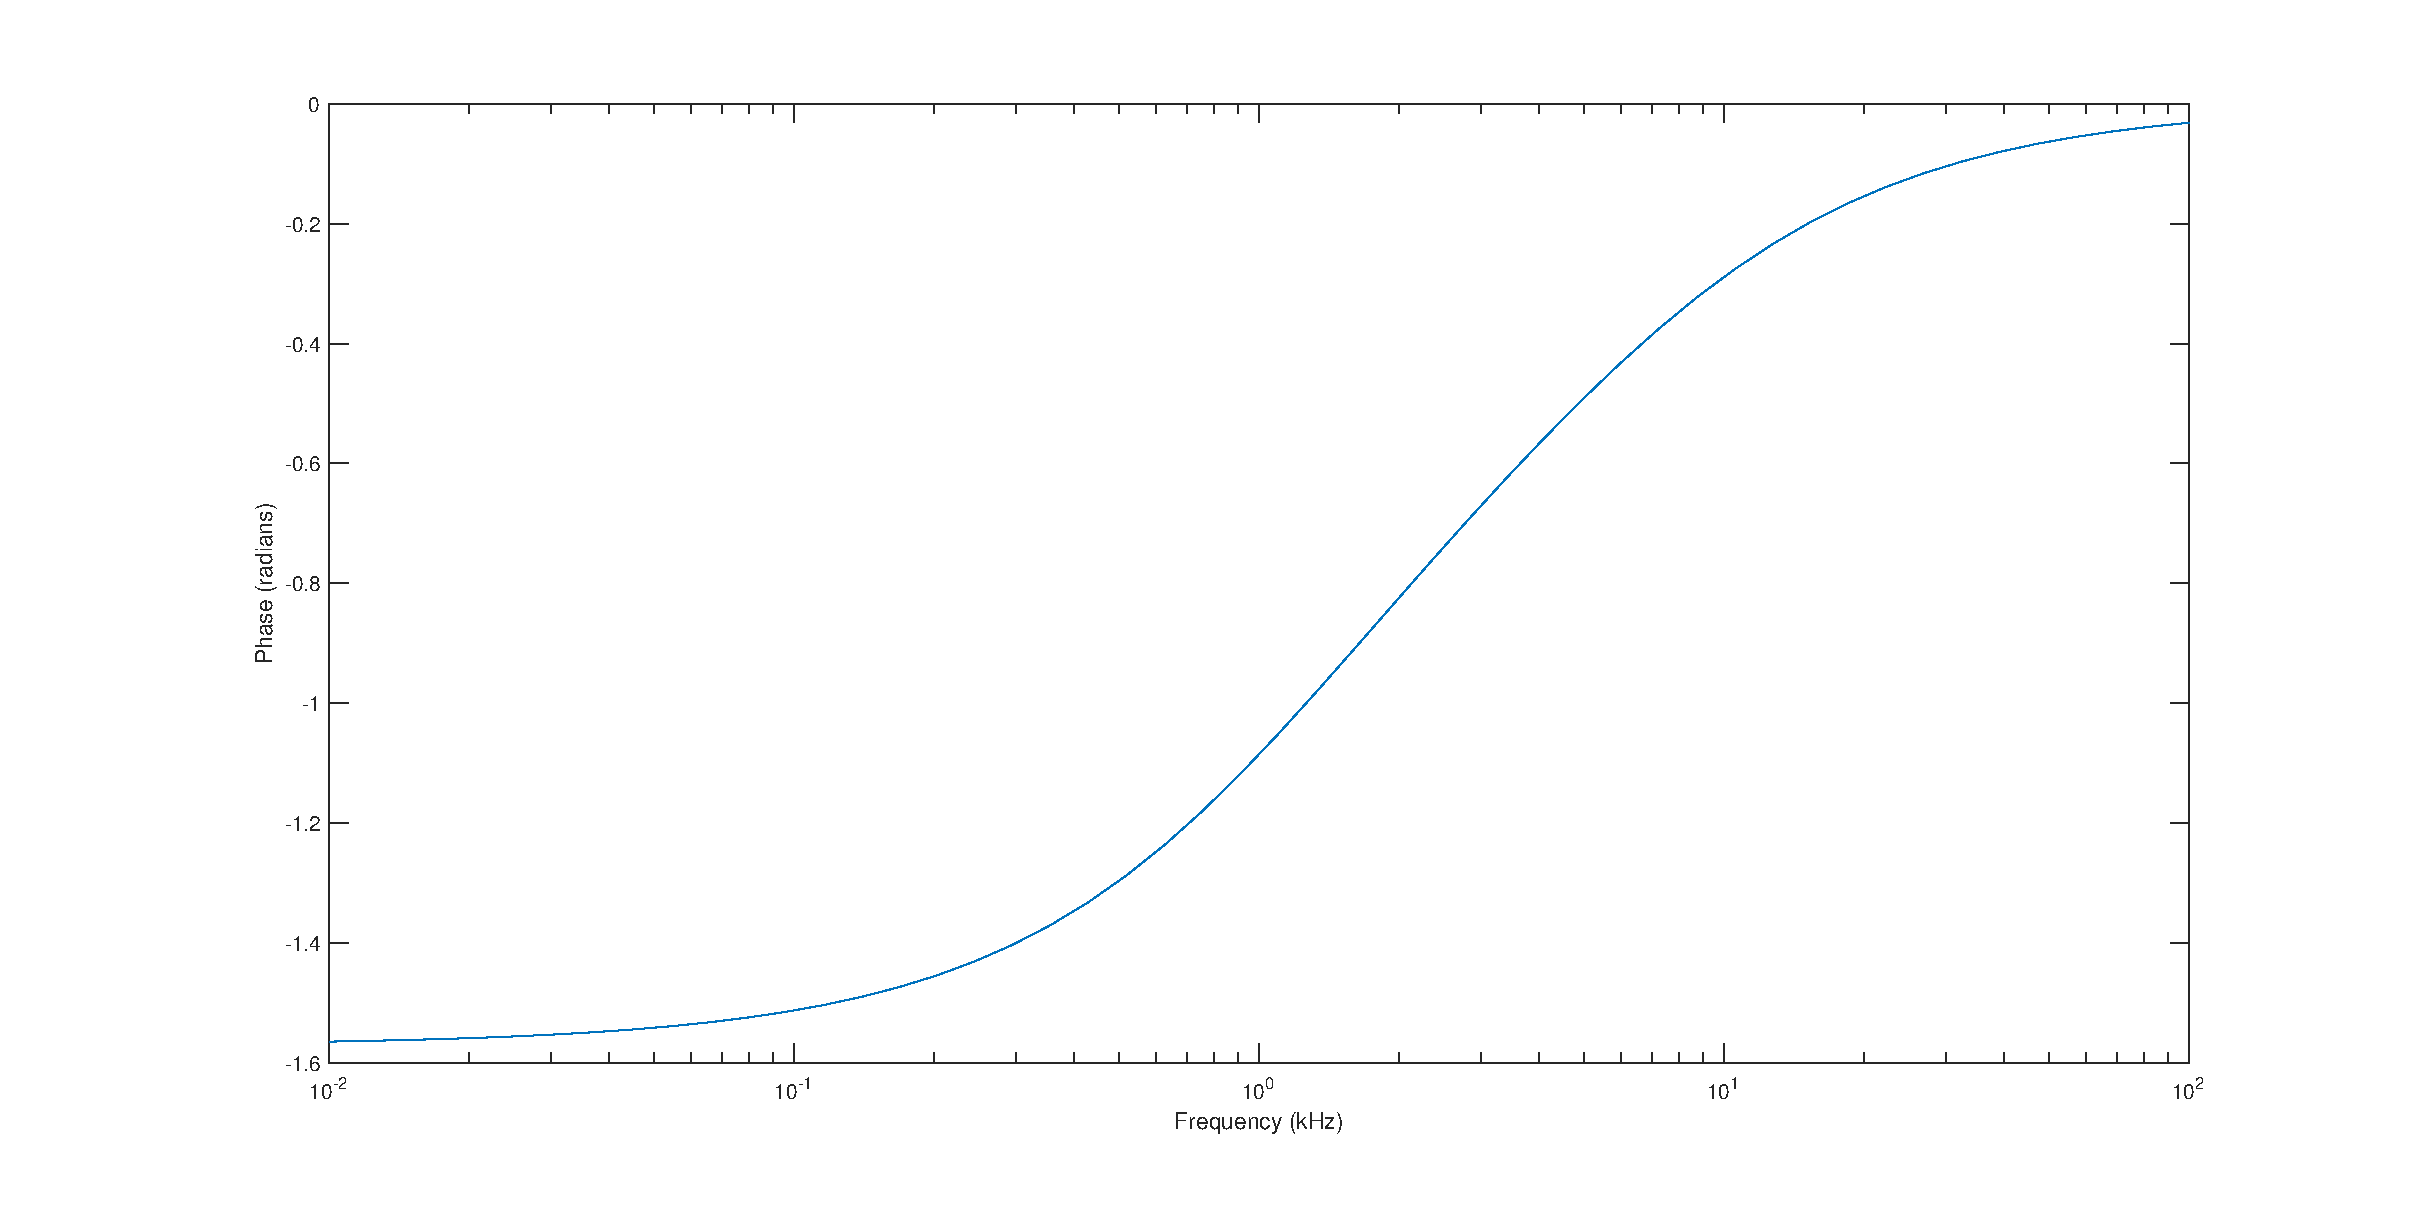
\includegraphics[width=\columnwidth]{4.eps}
        \end{column}
    \end{columns}
\end{frame}
\begin{frame}[fragile]{Total Impedance $Z$}{MATLAB Code}
    \inputminted[frame=single,bgcolor=bg,breaklines,breakanywhere,fontsize=\tiny]{matlab}{../Model/impedance.m}
\end{frame}
\begin{frame}{Time-Averaged Velocity}
    Given $v_{DL}=\frac{\lambda_D\rho_{DL}E_{HL}}{\eta}$, how to derive its time-averaged value?\\
    Note that both $\rho_{DL}=\frac{\Psi_{DL}\varepsilon}{\lambda_D}$ and $E_{HL}=-\frac{\Psi}{\sqrt{k}(1+k)}\frac{\frac{i\omega\varepsilon\pi}{2\lambda_D\sigma}}{(1+\frac{i\omega\varepsilon\pi x}{2\lambda_D\sigma})^2}$ have the part $\Psi=\Psi_0\exp{i\omega t}$.
    Remind the method we use in calculating the time-averaged power:\\
    \[<P>=\frac{1}{T}\int_0^T{V_0I_0\cos{(\omega t+\phi_1)}\cos{(\omega t+\phi_2)}\mathrm{d}t}\]
    Using the formula\\
    \[\cos{(A+B)=\cos{A}\cos{B}-\sin{A}\sin{B}}\]
    we have\\
    \footnotesize{\[<P>=\frac{1}{T}\int_0^T{V_0I_0(\cos{\omega t}\cos{\phi_1}-\sin{\omega t}\sin{\phi_1})(\cos{\omega t}\cos{\phi_2}-\sin{\omega t}\sin{\phi_2})\mathrm{d}t}\]}
\end{frame}
\begin{frame}{Time-Averaged Velocity}
    \[
        \begin{aligned}
            <P>=&\frac{1}{T}\int_0^T(\cos^2{\omega t}\cos{\phi_1}\cos{\phi_2}+\sin^2{\omega t}\sin{\phi_1}\sin{\phi_2}\\
            &-\cos{\omega t}\sin{\omega t}(\cos{\phi_1}\sin{\phi_2}+\cos{\phi_2}\sin{\phi_1}))\mathrm{d}t
        \end{aligned}
    \]
    Since $\int_0^T{\sin^2{\omega t}}=\frac{T}{2}$, $\int_0^T{\cos^2{\omega t}}=\frac{T}{2}$, and $\int_0^T{\sin{\omega t}\cos{\omega t}}=0$,\\
    \[<P>=\frac{1}{2}V_0I_0\left(\cos{\phi_1}\cos{\phi_2}+\sin{\phi_1}\sin{\phi_2}\right)=\frac{1}{2}V_0I_0\cos{(\phi_1-\phi_2)}\]
    Thus,
    \[<P>=\frac{1}{2}\mathrm{Re}\left(I_0V_0e^{i\phi_1}e^{-i\phi_2}\right)=\frac{1}{2}\mathrm{Re}\left(\tilde{I}_0\tilde{V}_0^*\right)\]
    Similarly, we can write
    \[<v_{DL}>=\frac{1}{2}\mathrm{Re}\{\frac{\lambda_D\rho_{DL}E_{HL}^*}{\eta}\}\]
\end{frame}
\section{Improved Model}
\begin{frame}{Improved Model}{Electrical Prolem}
    Let's start from Poisson's equation:
    \[\nabla^2\phi=\frac{\rho}{\varepsilon}=\frac{e(n_--n_+)}{\varepsilon}\]
    and the continuity equation (charge conservation equation):
    \[\nabla\cdot\bm{J}=-\frac{\partial\rho}{\partial t}\]
    Remind in VE320 Chapter 5: Carrier Transport Phenomena 5.2 Carrier Diffusion 5.2.2 Total Current Density Eq. (5.36) is the sum of electric drift and diffusion density:
    \[J=en\mu_nE+ep\mu_pE+eD_n\nabla n-eD_p\nabla p\]
    Adding drift due to the fluid motion:
    \[\bm{J}_\pm=\mp en_\pm\mu\nabla\phi-eD\nabla n+en_\pm\bm{u}\]
    where $\bm{u}$ is the liquid velocity, $\rho$ is the (volume) charge density.
\end{frame}
\begin{frame}{Electrical Prolem}{Scales and parameters}
    Here to simplify our calculation, we use a dimensional analysis technique called "nondimensionalization" or "scaling" in order to suggest that certain quantities are better measured relative to some appropriate unit that is especially useful for systems that can be described by differential equations.\\
    Next, we plan to use this method (or not) to calculate the electric field.
\end{frame}
\begin{frame}{Electrical Prolem}
    The electrical potential in the bulk electrolyte satisfies Laplace's Equation
    \[\nabla^2\Phi=0\]
    $\Phi$ is the potential just outside the double layer.\\
    Low voltage assumption: the voltage drop across the double layer is linear to the surface charge $\frac{\partial q_s}{\partial t}=-\sigma E_y$. The surface charge conservation equation:
    \[\sigma\frac{\partial\Phi}{\partial y}=i\omega C_{DL}(\Phi-V_j)\]
    Note that different from previous definition, here $C_{DL}$ is the capacitance per unit of \textbf{area} of the total double layer.\\
    Boundary condition at the interface between the electrolyte and the glass:
    \[(\sigma+i\varepsilon\omega)\frac{\partial\Phi}{\partial y}=(\sigma_g+i\varepsilon_g\omega)\frac{\partial\Phi_g}{\partial y}\]
\end{frame}
\begin{frame}{Electrical Prolem}
    Remind the Ampère's circuital law with Maxwell's addition (differential equations SI convention):
    \[\nabla\times\bm{H}=\bm{J}_f+\frac{\partial\bm{D}}{\partial t}\]
    Since the electric potential is alternating as $\bm{\Phi}=\bm{\Phi}_0\exp{\left(i\omega t\right)}$,
    \[\bm{j}+\frac{\partial\bm{D}}{\partial t}=\bm{j}+i\varepsilon\omega\frac{\partial\bm{\Phi}}{\partial y}=(\sigma+i\varepsilon\omega)\frac{\partial\bm{\Phi}}{\partial y}\]
    not to be confused with the electromagnetic wave $E=E_0\exp{(i(\bm{k}\cdot\bm{r})-\omega t)}$, which leads to $\sigma-i\varepsilon\omega$.
\end{frame}
\begin{frame}{Electrical Prolem}
    \begin{table}[H]
        \begin{tabular}{|c|c|}
            \toprule
            Material&Conductivity $\sigma$ at 20 $^\circ$C (S/m)\\
            \midrule
            Glass&$10^{-15}$ to $10^{-11}$\\
            Sea water&4.8\\
            Drinking water&$5\times10^{-4}$ to $5\times10^{-2}$\\
            Deionized water&$4.2\times10^{-5}$\\
            \bottomrule
        \end{tabular}
    \end{table}
    Since $\varepsilon_g\ll\varepsilon$ and $\omega\ll\frac{\sigma}{\varepsilon}$, we can simplify the equation to
    \[\frac{\partial\Phi}{\partial y}=0\]
    Besides,
    \[\int_{-\frac{L}{2}}^{-\frac{L}{2}}{\frac{\partial\Phi}{\partial y}\mathrm{d}x}=0\]
\end{frame}
\begin{frame}{Fluid Dynamic}
    Debye-Hückel theory: surface capacitance
    \[C_{DL}=\frac{\varepsilon}{\lambda_D}\]
    Helmholtz-Smoluchowski formula: electro-osmotic slip velocity
    \[u=\frac{\varepsilon\Delta\Phi}{\eta}E_x=-\frac{\varepsilon\Delta\Phi}{\eta}\frac{\partial\Phi}{\partial x}\]
    Using the same strategy introduced before, the time-averaged horizontal fluid velocity at the interface between the double layer and the bulk is
    \[<u>=-\frac{\varepsilon}{2\eta}\mathrm{Re}\left[\Delta\Phi\frac{\partial\Phi^*}{\partial x}\right]=-\frac{\varepsilon}{2\eta}\Lambda\mathrm{Re}\left[\Delta\Phi_{DL}\frac{\partial\Phi^*}{\partial x}\right]=-\frac{\varepsilon}{2\eta}\Lambda\frac{\partial}{\partial x}|\Phi-V_j|^2\]
    $\Phi$ is the potential just outside the double layer; $V_j$ is the potential applied to electrode $j$; $\Phi_{DL}$ is the total double layer potential drop.
\end{frame}
\begin{frame}{Fluid Dynamic}{The solution in the diffuse layer}
    The slip electro-osmotic velocity
    \[<u>=-\frac{\varepsilon}{2\eta}\Lambda\frac{\partial}{\partial x}\left[(\Phi-V_j)(\Phi-V_j)^*\right]\]
    where $\Lambda$ is the ratio of the diffuse double layer impedance to the total double layer impedance given by
    \[\Lambda=\frac{(i\omega C_{d})^{-1}}{(i\omega C_{DL})^{-1}}=\frac{C_s}{C_s+C_d}\]
    where $C_d$ and $C_s$ are the capacitances of the diffuse layer and the Stern or compact layer respectively. Boundary condition:
    \[\sigma\frac{\partial\Phi}{\partial y}=i\omega C_{DL}(\Phi-\Phi_g)=i\varepsilon_g\omega\frac{\partial\Phi_g}{\partial y}\]
\end{frame}
\begin{frame}{Fluid Dynamic}{The solution in the bulk}
    Incompressible Navier-Stokes equations (convective form)
    \includesvg{1\columnwidth}{7-rasterized}
    % 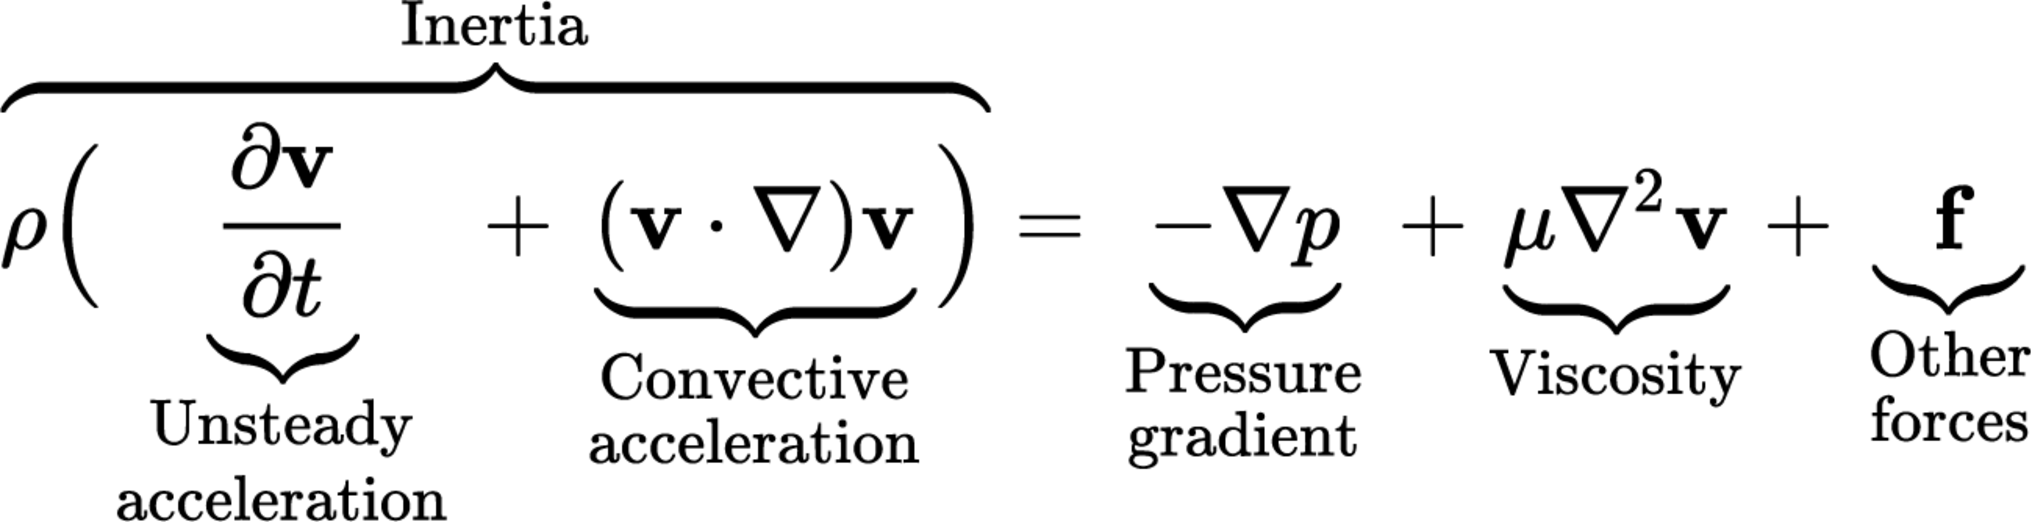
\includegraphics[width=0.8\linewidth]{7-rasterized.pdf}
    For microsystems, the Reynolds number $\mathrm{Re}=\frac{\rho VD}{\eta}=\frac{VD}{\nu}$ is very small ($D\sim2\times10^{-5}$m, $V\sim5\times10^{-4}$m/s, $\nu=\mu/\rho\sim10^{-6}\,\mathrm{m^2/s}$, $\mathrm{Re}\sim10^{-2}$), so inertial terms (and the externally applied body forces) can be neglected:
    \[\eta\nabla^2\bm{u}-\nabla p=0\]
    \[\nabla\cdot\bm{u}=0\]
    Next, we plan to solve the differential equations.
\end{frame}
\section{COMSOL Simulation}
\begin{frame}{COMSOL Simulation}{Parameters}
    To simulate our model, we mainly referred to a COMSOL sample "Electroosmotic Micromixer".
    Our parameters are:
    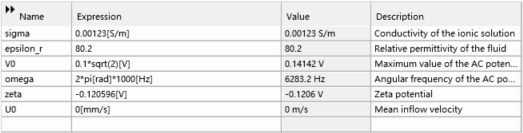
\includegraphics[width=0.8\textwidth]{8.png}
\end{frame}
\begin{frame}{COMSOL Simulation}{Geometry}
    Our geometry is:
    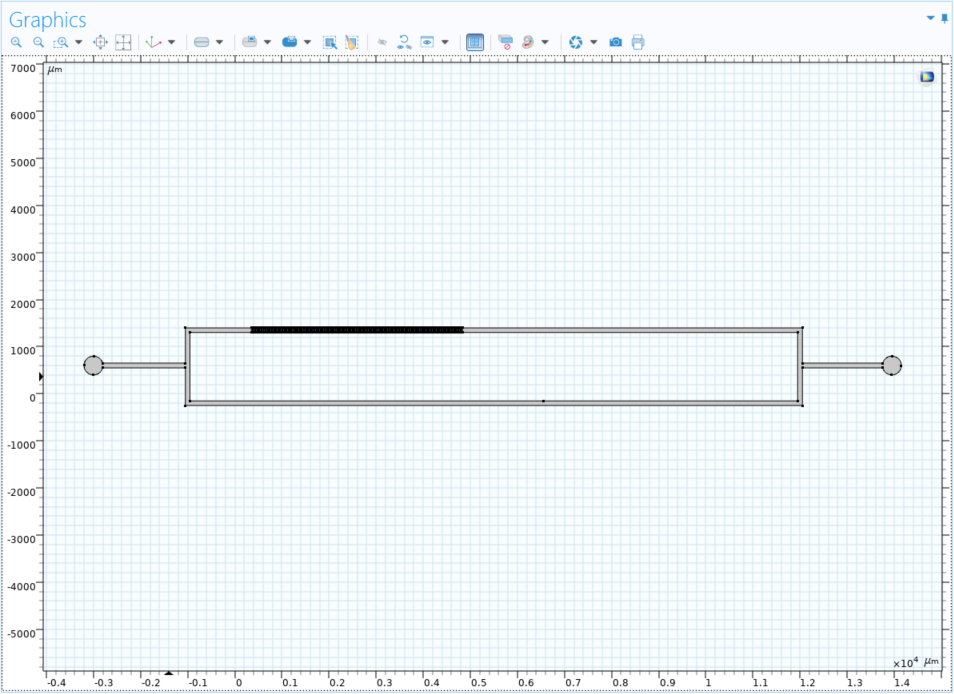
\includegraphics[width=0.8\textwidth]{9.png}
\end{frame}
\begin{frame}{COMSOL Simulation}{Material}
    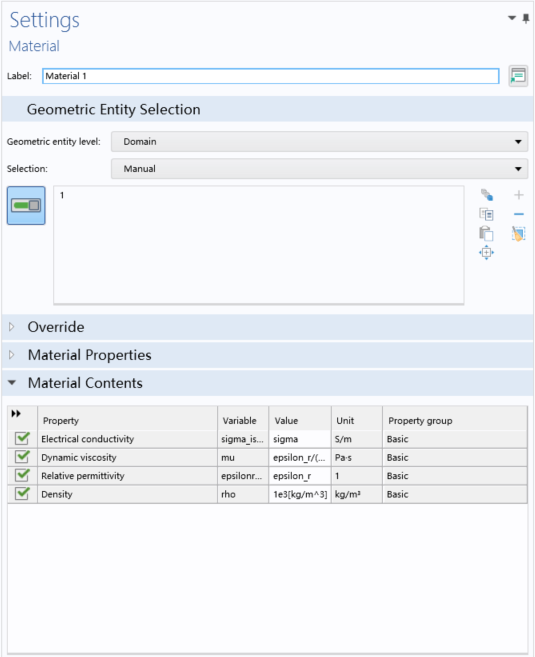
\includegraphics[width=0.6\textwidth]{10.png}
\end{frame}
\begin{frame}{Creeping Flow}{Wall ($U_{av}=U0$)}
    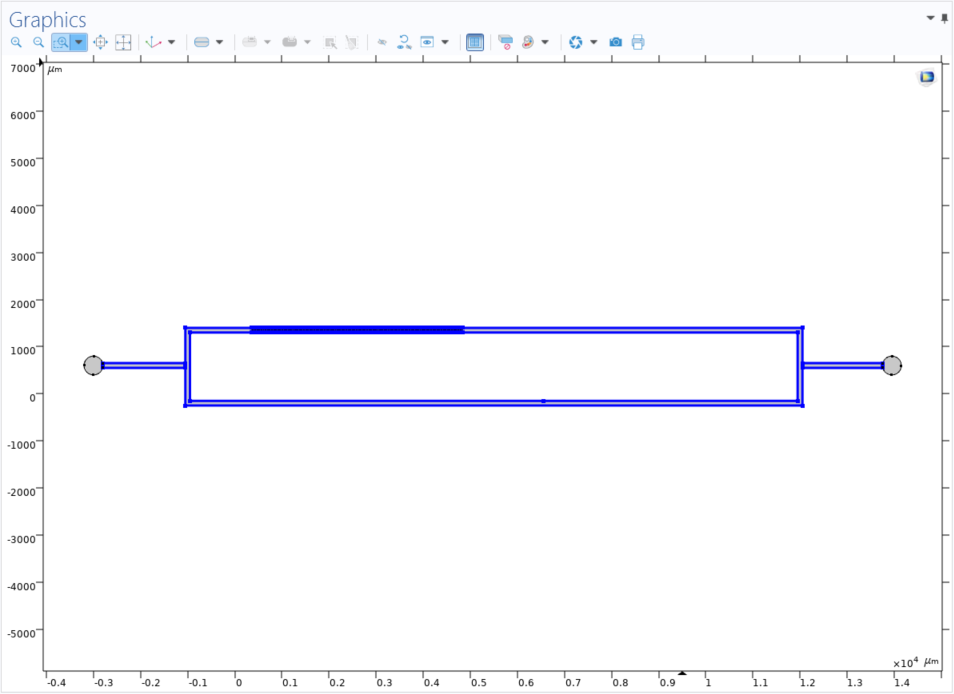
\includegraphics[width=0.8\textwidth]{11.png}
\end{frame}
\begin{frame}{Creeping Flow}{Inlet}
    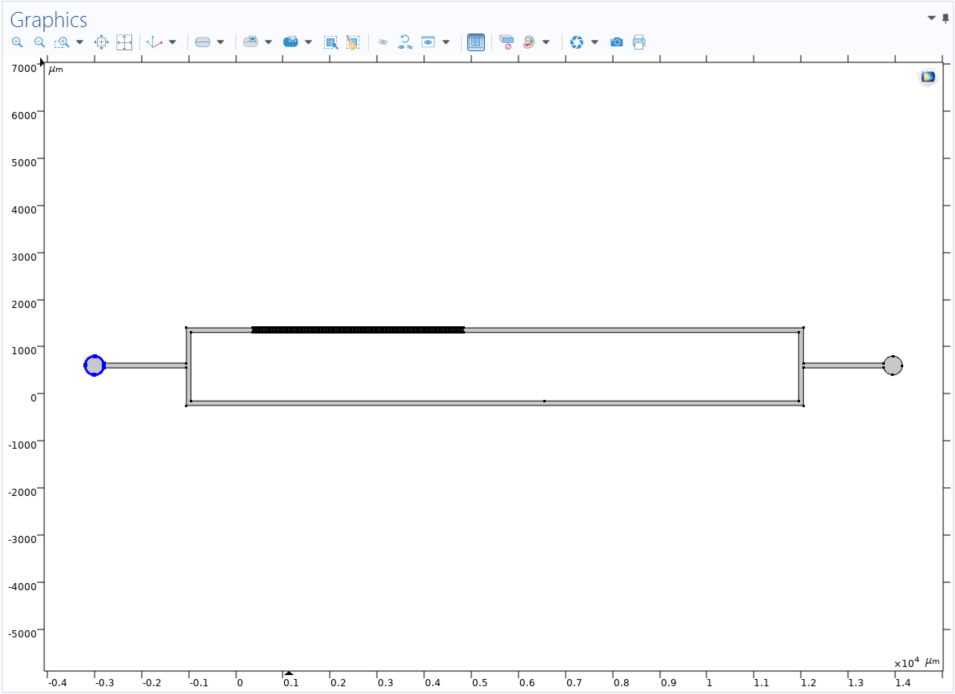
\includegraphics[width=0.8\textwidth]{12.png}
\end{frame}
\begin{frame}{Creeping Flow}{Outlet}
    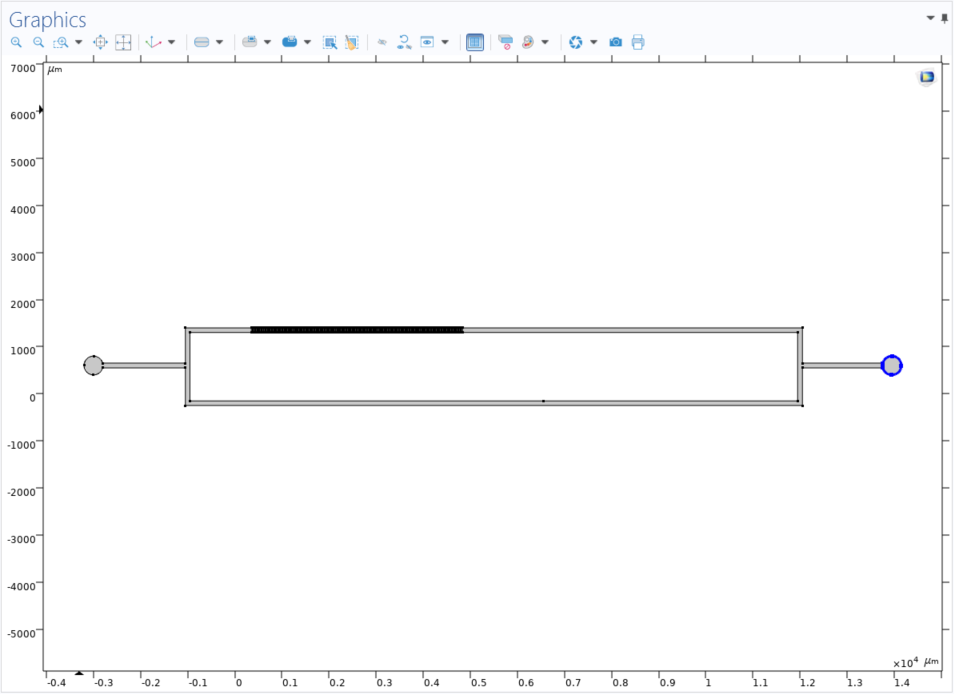
\includegraphics[width=0.8\textwidth]{13.png}
\end{frame}
\begin{frame}{Electric Currents}{Electric Potential 1 ($V_0=V0$)}
    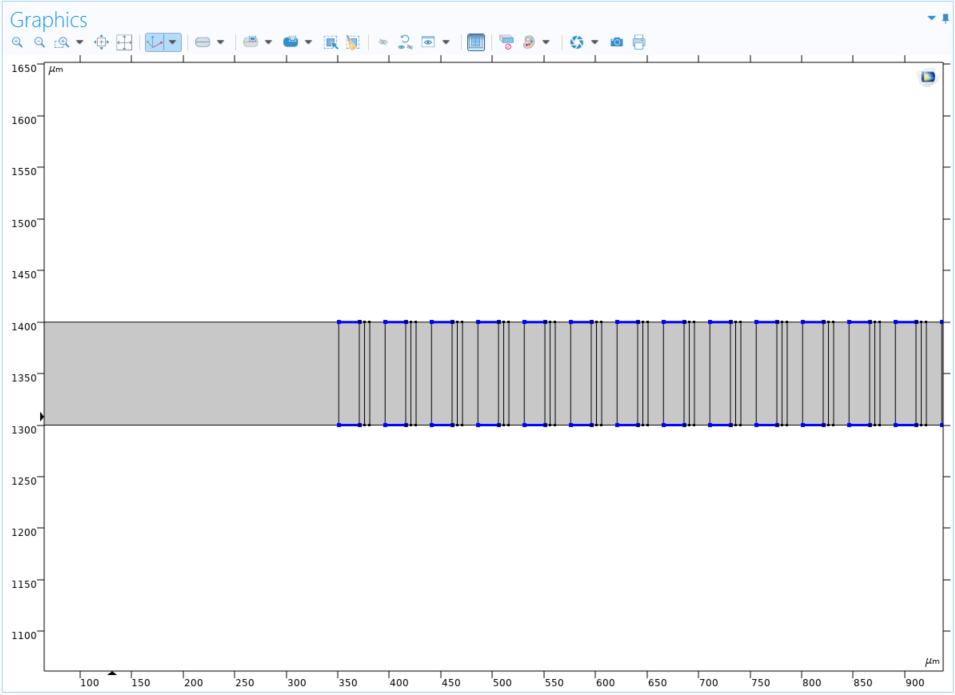
\includegraphics[width=0.8\textwidth]{14.png}
\end{frame}
\begin{frame}{Electric Currents}{Electric Potential 2 ($V_0=-V0$)}
    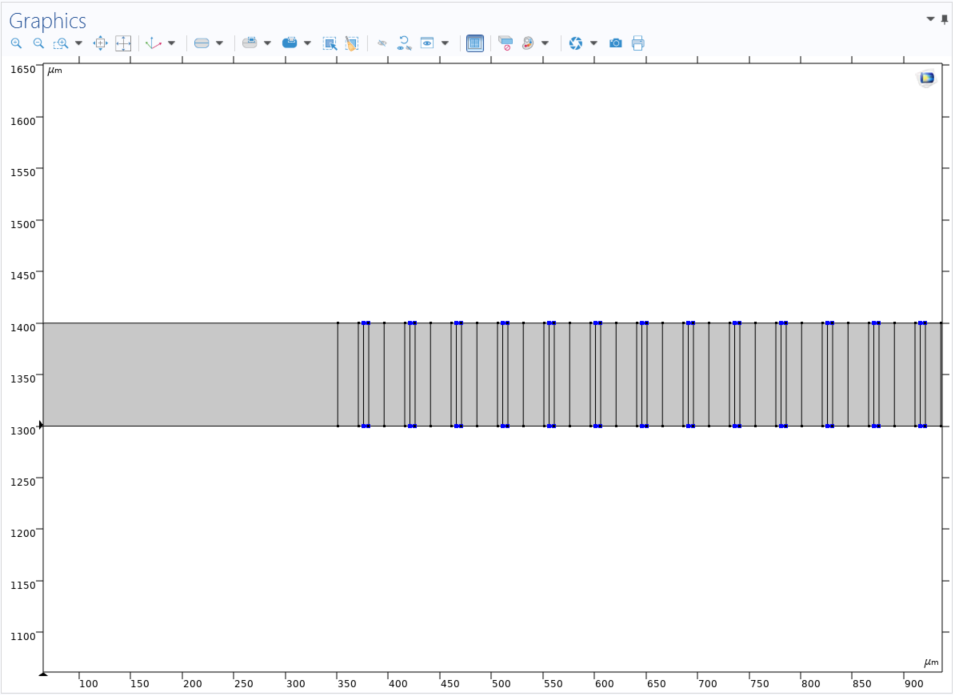
\includegraphics[width=0.8\textwidth]{15.png}
\end{frame}
\begin{frame}{COMSOL Simulation}{Material}
    Then, we set up a study using time-dependent solver to solve the fluid flow. After computing, we can derive the results including:
    \begin{itemize}
        \item Velocity, streamlines
        \item Electric potential
    \end{itemize}
    Next, we plan to modify the original layout in GDS file in AutoCAD to fit the COMSOL geometry requirements.
\end{frame}
\begin{frame}
    \begin{center}
        Thanks!
    \end{center}
\end{frame}
\end{document}